\documentclass[tikz,border=2pt]{standalone}
\usepackage{amsmath}
\usetikzlibrary{arrows.meta}
\begin{document}
% The four ways to draw k = 3 of n = 10 tickets: ordered with replacement 10^3 = 1000, ordered
% without 720, unordered without C(10,3) = 720/3! = 120, unordered with C(12,3) = 220.
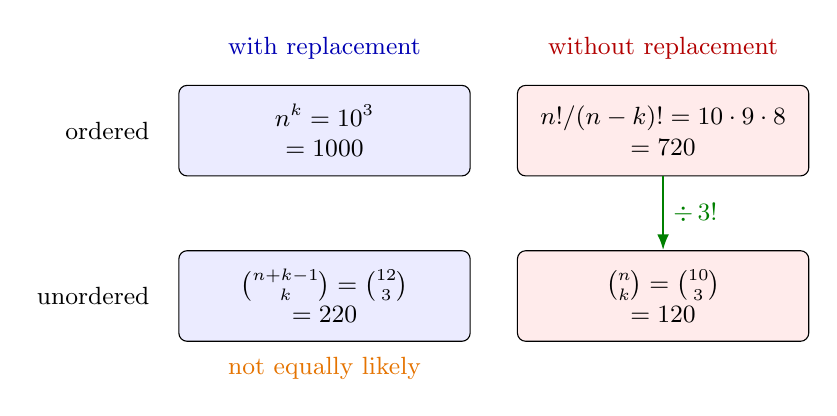
\begin{tikzpicture}[font=\small, >={Latex[length=2mm]},
  cell/.style={draw, rounded corners=3pt, minimum width=3.7cm, minimum height=1.15cm, align=center}]
  % column headers
  \node[blue!70!black] at (0,1.05) {with replacement};
  \node[red!70!black] at (4.3,1.05) {without replacement};
  % row headers
  \node[anchor=east] at (-2.1,0) {ordered};
  \node[anchor=east] at (-2.1,-2.1) {unordered};
  % cells
  \node[cell, fill=blue!8] (ow) at (0,0) {$n^k=10^3$\\$=1000$};
  \node[cell, fill=red!8] (oo) at (4.3,0) {$n!/(n-k)!=10\cdot9\cdot8$\\$=720$};
  \node[cell, fill=blue!8] (uw) at (0,-2.1) {$\binom{n+k-1}{k}=\binom{12}{3}$\\$=220$};
  \node[cell, fill=red!8] (uo) at (4.3,-2.1) {$\binom{n}{k}=\binom{10}{3}$\\$=120$};
  % dividing out the k! orders works only without replacement
  \draw[->, green!50!black, thick] (oo.south) -- node[right, green!50!black] {$\div\,3!$} (uo.north);
  \node[orange!90!black, anchor=north] at (0,-2.75) {not equally likely};
\end{tikzpicture}
\end{document}
